\section{Solution réalisée}
Une étape essentielle dans tout système électrique réside premièrement dans son câblage. Le but a été d'avoir un câblage le plus propre et pratique possible.
La figure \ref{cablage_kit_pas_annoté}, ci-dessous, est une photo du kit sans les annotations pour mieux voir le câblage effectué. Sur la prochaine page, on retrouve cette photo mais avec les annotations et les explications en détail des différents câbles.
\begin{figure}[H]
    \begin{center}
        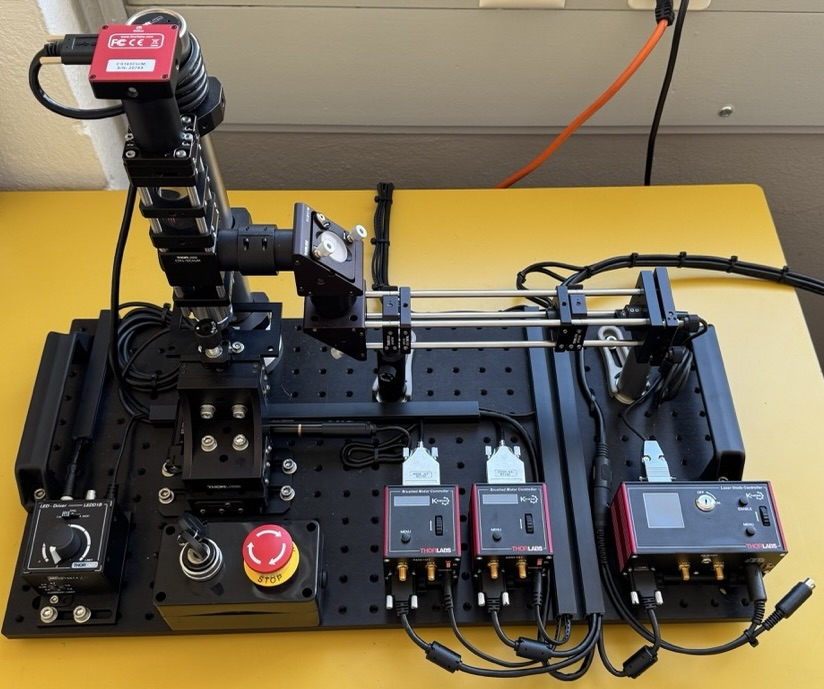
\includegraphics[width=\textwidth]{assets/figures/Cablage_du_kit/Cablage_vierge.jpeg}
    \end{center}
    \caption{Câblage du kit sans annotations}
    \label{cablage_kit_pas_annoté}
\end{figure}

\newpage
Ci-dessous, une photo du câblage avec des annotations pour une bonne compréhension du travail réalisé (voir Figure \ref{cablage_kit_annoté}).


\begin{figure}[H]
    \begin{center}
        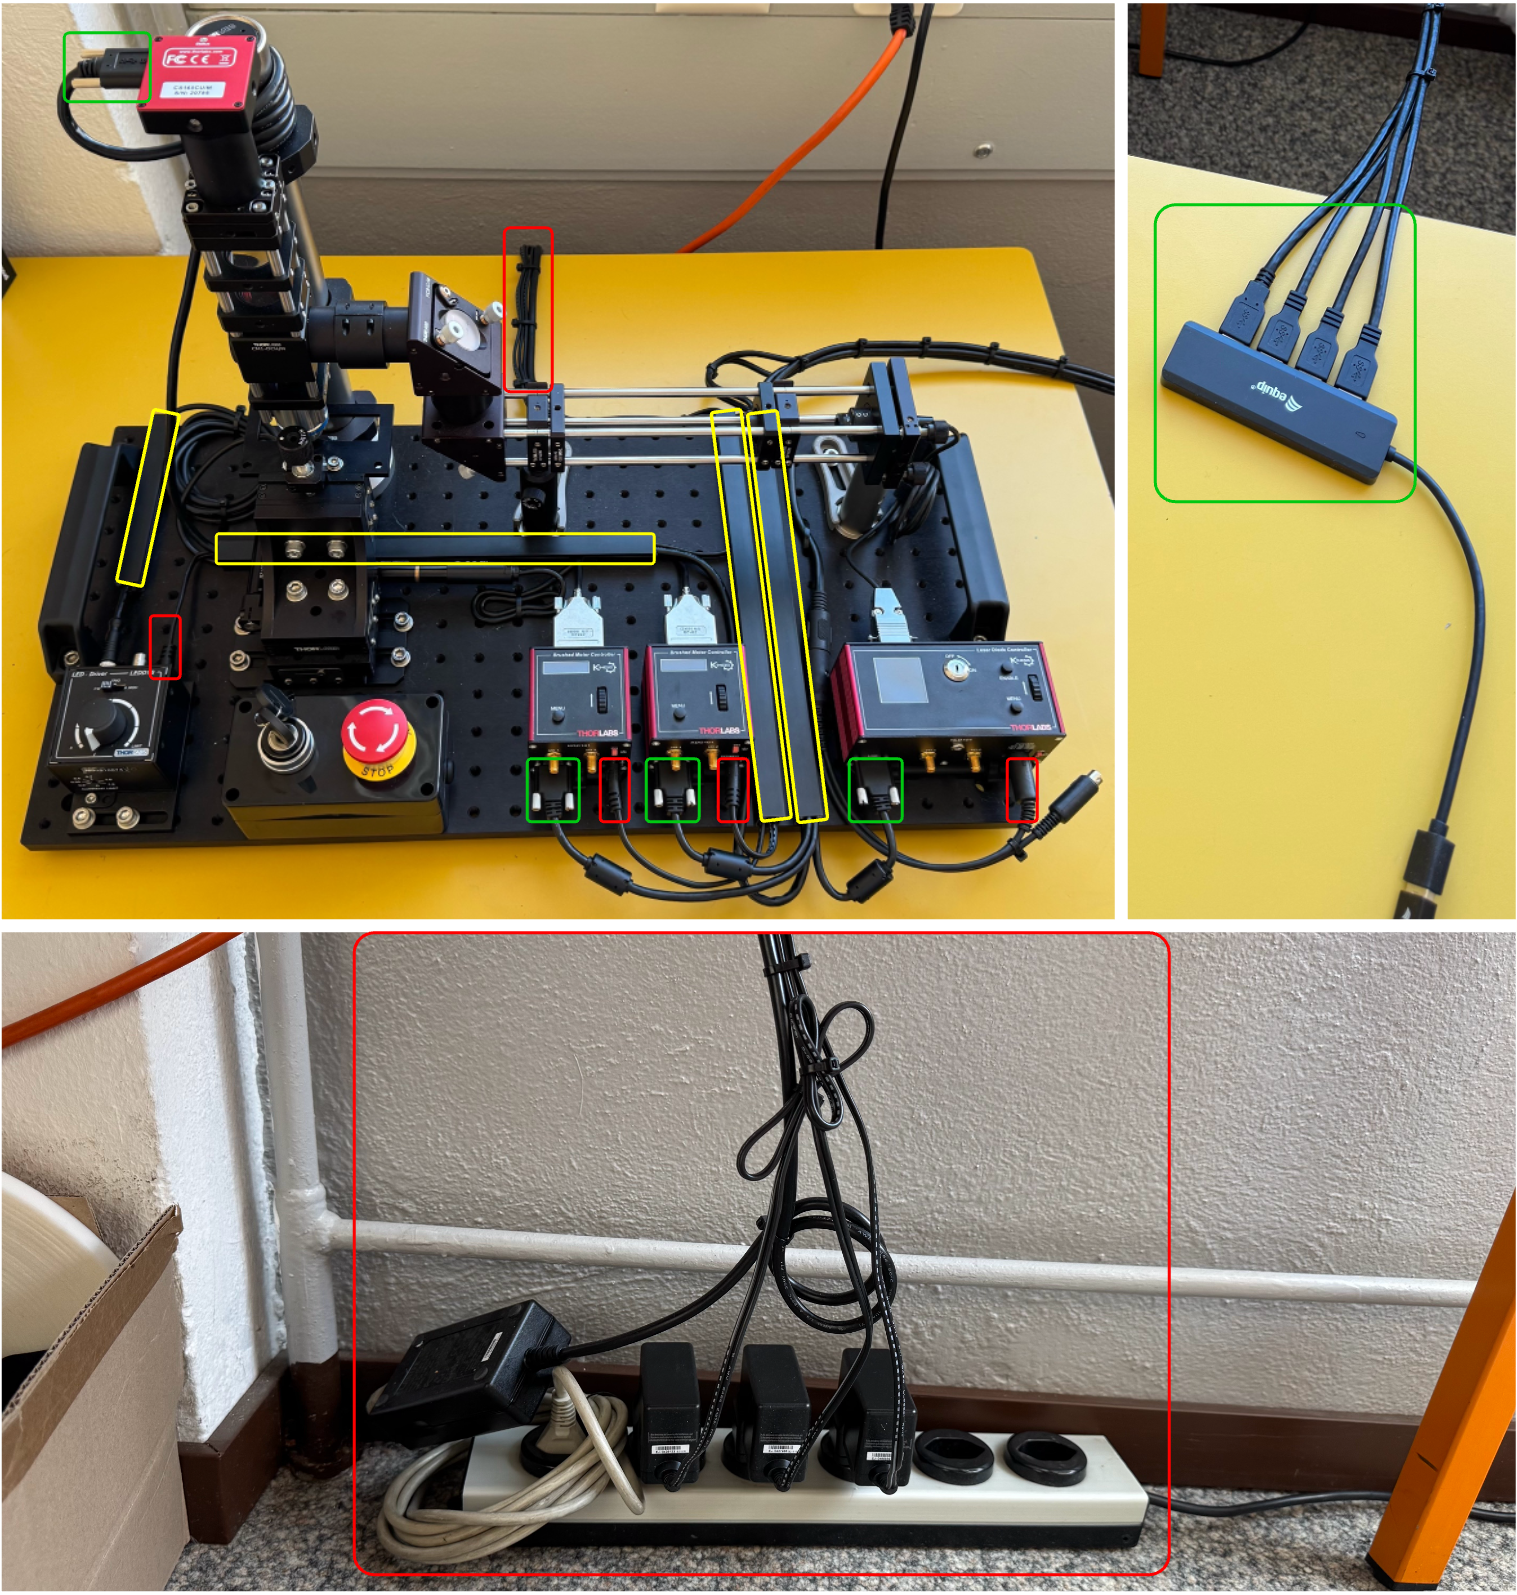
\includegraphics[width=0.9\textwidth]{assets/figures/Cablage_du_kit/Cablage_annote.png}
    \end{center}
    \caption{Câblage du kit avec annotations}
    \label{cablage_kit_annoté}
\end{figure}

Du point de vue de la propreté, on peut apercevoir, en \textcolor[RGB]{230, 230, 0}{jaune}, que des goulottes ont été installées. Celles-ci permettent de rassembler plusieurs câbles et qu'ils tiennent en place.

Les encadrés en \textcolor{red}{rouge} sont les 4 alimentations. Il y'a une alimentation pour :
\begin{itemize}
    \item Les 2 drivers des servomoteurs.
    \item Le driver du laser.
    \item Le driver de la LED.
\end{itemize}

En complément des alimentations, les encadrés en \textcolor[RGB]{0, 201, 18}{vert} sont les câbles permettant de communiquer avec les différents composants. La liste des câbles pour la communication ci-dessous :
\begin{itemize}
    \item 1 câble pour chaque driver de servomoteur, 2 au total.
    \item 1 câble pour le driver du laser.
    \item 1 câble pour la caméra.
\end{itemize}